\documentclass[conference]{IEEEtran}
\usepackage[T1]{fontenc}
\IEEEoverridecommandlockouts
\usepackage{cite}
\usepackage{amsmath,amssymb,amsfonts}
\usepackage{graphicx}
\usepackage{booktabs}
\usepackage{array}
\usepackage{flushend}
\usepackage{pifont}
\usepackage{xcolor}
\usepackage{tikz}
\usetikzlibrary{positioning,arrows.meta,calc,fit}
\usepackage[hidelinks]{hyperref}

\newcommand{\yes}{\ding{51}}
\newcommand{\prt}{$\sim$}
\newcommand{\no}{--}
\newcommand{\ind}{\mathbf{1}}
\newcommand{\ReplicationAbstract}{The all-listing source audit is complete, but its held-out model evaluation remains in progress; no completed replication or participant study is claimed.}
\newcommand{\ReplicationResults}{The source audit attempted all 302 listed securities and exported 253 histories; 200 non-development securities met the fixed eligibility conditions. At this manuscript snapshot, 74 held-out runs were complete, 6 had failed and 120 eligible runs remained pending. Table~\ref{tab:inclusion} records that status. Intermediate results are deliberately not used to claim replication. The bounded queue continues without changing the statistical rules; an updated manuscript can be rebuilt when the cohort finishes.}
\newcommand{\ReplicationConclusion}{Broader replication is underway on the source-audited eligible cohort; no final cross-stock performance claim is yet made.}
\hypersetup{pdftitle={From Daily Anomalies to Deviation Patterns: Liquidity-Aware, Explainable Market Evidence for Colombo Stock Exchange Investors},
pdfauthor={S. A. H. Samarathunga; K. C. S. Fernando; Harithra K; T. G. R. N. S. Wijesooriya; Kapila Dissanayaka; Mahima Weerasinghe}}

\makeatletter
\newcommand{\linebreakand}{\end{@IEEEauthorhalign}\hfill\mbox{}\par\mbox{}\hfill\begin{@IEEEauthorhalign}}
\makeatother
\begin{document}

\title{From Daily Anomalies to Deviation Patterns: Liquidity-Aware, Explainable Market Evidence for Colombo Stock Exchange Investors}

\author{
\IEEEauthorblockN{S. A. H. Samarathunga}
\IEEEauthorblockA{\textit{Faculty of Computing}\\
\textit{Sri Lanka Institute of Information}\\\textit{Technology}\\
Malabe, Sri Lanka\\
hasanthasamarthunga89@gmail.com}
\and
\IEEEauthorblockN{K. C. S. Fernando}
\IEEEauthorblockA{\textit{Faculty of Computing}\\
\textit{Sri Lanka Institute of Information}\\\textit{Technology}\\
Malabe, Sri Lanka\\
chanosadunika02@gmail.com}
\and
\IEEEauthorblockN{Harithra K}
\IEEEauthorblockA{\textit{Faculty of Computing}\\
\textit{Sri Lanka Institute of Information}\\\textit{Technology}\\
Malabe, Sri Lanka\\
harithrakanna@gmail.com}
\linebreakand
\IEEEauthorblockN{T. G. R. N. S. Wijesooriya}
\IEEEauthorblockA{\textit{Faculty of Computing}\\
\textit{Sri Lanka Institute of Information}\\\textit{Technology}\\
Malabe, Sri Lanka\\
ruchiniwijesooriya@gmail.com}
\and
\IEEEauthorblockN{Kapila Dissanayaka}
\IEEEauthorblockA{\textit{Faculty of Computing}\\
\textit{Sri Lanka Institute of Information}\\\textit{Technology}\\
Malabe, Sri Lanka\\
kapila.d@sliit.lk}
\and
\IEEEauthorblockN{Mahima Weerasinghe}
\IEEEauthorblockA{\textit{Faculty of Computing}\\
\textit{Sri Lanka Institute of Information}\\\textit{Technology}\\
Malabe, Sri Lanka\\
mahima.w@sliit.lk}
}

\maketitle

\begin{abstract}
Daily price alerts do not explain whether a falling stock has experienced an isolated shock or a sustained departure from its recent pattern. We evaluate a market-evidence workflow for Colombo Stock Exchange investors, combining expected prices, participation-adjusted deviations, calibrated alerts and an offline deviation-pattern extension. Reproduced development experiments use John Keells Holdings and Browns Investments histories through August 2026. After correcting the rolling scale calculation, robust residuals give the highest observed daily harmonic mean of precision and recall, 0.786 and 0.400, against return-based proxy labels. A separate fixed-budget combined rule flags all six documented stock--crisis cases, with 1.93 and 1.98 out-of-episode alerts per 100 sessions. Pattern rules calibrated on earlier observations label five cases but miss two substantial Browns declines, demonstrating why continuous profile statistics should accompany labels. Persistence outperforms the preserved three-month forecasts; attribution fidelity depends strongly on the score being explained. \ReplicationAbstract\ The contribution is an inspectable evidence framework, not established forecasting superiority, causal event identification or validated investor comprehension.
\end{abstract}

\begin{IEEEkeywords}
Colombo Stock Exchange, anomaly detection, deviation patterns, explainability, investor decision support
\end{IEEEkeywords}

\section{Introduction}
Participation in the CSE is narrow: in 2025 the Securities and Exchange Commission (SEC) chairman reported that only 5\% of 14.41 million adults held Central Depository System accounts and linked this to low financial literacy~\cite{dailymirror_literacy2025}. Prospective investors face prices that move sharply during crises, such as the trading closure after the 2019 Easter attacks~\cite{ft_easter2019}, the seven-week COVID-19 closure in 2020~\cite{morning_covid2020} and the five-day SEC-ordered halt during the 2022 sovereign crisis~\cite{bs_halt2022}. A forecast line alone does not tell a new investor whether today's fall is ordinary noise, an isolated shock, or part of a sustained decline.

The AI-Powered Stock Market Insight Generator addresses this with four components: market behaviour (this paper), financial-report interpretation, news and sentiment, and global-factor risk. A fusion layer combines them into one plain-language outlook in English, Sinhala or Tamil, without buy or sell instructions. This paper evaluates the market component and asks two questions. Does a participation-aware deviation rule detect unusual CSE movements better than simple baselines? Can deviations be summarised into patterns that describe how a stock behaves through stress?

Contributions are: (i) an evaluated participation-adjusted residual and independent band alert; (ii) an offline pattern extension using past-only robust residuals, cumulative-sum (CUSUM) and exponentially weighted moving-average (EWMA) monitors; (iii) reproduced development ablations, uncertainty reporting and documented-event case studies; (iv) held-out surrogate-fidelity and explanation-stability checks; and (v) a source-audited replication pipeline with a versioned participant-study protocol. Completed experiments and planned evaluation are distinguished throughout. The pattern extension is research code; it is not claimed to be fully deployed in the investor interface.

\section{Related Work}
Long short-term memory (LSTM) networks support sequence learning~\cite{hochreiter1997}, but forecasts require persistence comparisons~\cite{hyndman2021}. Anomaly definitions and labels matter~\cite{chandola2009}; Isolation Forest~\cite{liu2008}, Z-scores and precision--recall measures~\cite{saito2015} provide references. Amihud relates returns to monetary volume~\cite{amihud2002}; our score uses a model price residual and share volume. CUSUM~\cite{page1954} and EWMA~\cite{roberts1959} monitor shifts. Shapley additive explanations (SHAP) and Tree SHAP~\cite{lundberg2017,lundberg2020} explain a random-forest surrogate~\cite{breiman2001}.

\begin{table*}[!t]
\caption{Feature-Level Comparison With Existing Studies and Systems}
\label{tab:compare}
\centering
\footnotesize
\setlength{\tabcolsep}{2.7pt}
\renewcommand{\arraystretch}{1.05}
\begin{tabular}{@{}l l l c c c c c c c l@{}}
\toprule
Work & Market and data & Main purpose & Flag & Vol. & Patt. & Expl. & Stab. & Naive & Unc. & Reported evaluation \\
\midrule
Sirimevan et al.~\cite{sirimevan2019} & DJIA; prices, tweets, news & LSTM price ensemble & \no & \no & \no & \no & \no & \no & \no & RMSE, undefined accuracy \\
Kumarasinghe et al.~\cite{kumarasinghe2019} & 12 CSE firms; macro, news & LSTM/RNN prediction & \no & \no & \no & \prt & \no & \no & \no & MAE, MAPE, RMSE \\
Nanayakkara et al.~\cite{nanayakkara2021} & CSE; prices & Prediction, portfolio & \no & \no & \no & \no & \no & \no & \no & Not named in abstract \\
Vithushan, Kethmi~\cite{vithushan2025} & S\&P SL20 index & ARIMA vs.\ LSTM & \no & \no & \no & \no & \no & \no & \no & MAE, MAPE, RMSE \\
Golmohammadi et al.~\cite{golmohammadi2014} & US; hourly; SEC cases & Manipulation classes & \yes & \no & \no & \no & \no & \prt & \no & Litigation labels; F2 \\
Cao et al.~\cite{cao2015} & NASDAQ, LSE ticks & HMM anomaly states & \yes & \no & \no & \no & \no & \no & \no & Tick sets, simulations \\
AIMM-X~\cite{neela2026} & 24 US tickers & Integrity triage & \yes & \prt & \prt & \yes & \no & \no & \no & No ground truth \\
Nasdaq SMARTS~\cite{ciro_smarts,dailymirror_sec2024} & Orders, trades & Regulator alerts & \yes & \prt & \no & \no & \no & \no & \no & Not public \\
Simply Wall St~\cite{simplywallst_snowflake} & Listed firms & Fundamental checks & \no & \no & \no & \prt & \no & \no & \no & Not reported \\
\midrule
\textbf{This work} & CSE; daily OHLCV & Market evidence & \yes & \yes & \yes & \yes & \yes & \yes & \yes & Past-only labels; 3 episodes \\
\bottomrule
\end{tabular}

\vspace{2pt}
\parbox{\textwidth}{\scriptsize Flag: unusual-movement alert. Vol.: participation enters the alert. Patt.: sustained-deviation monitoring. Expl.: factor-level explanation. Stab.: explanation stability measured. Naive: persistence or trivial reference. Unc.: ranges with empirical coverage. \yes\ described in the cited source; \prt\ partial (regression factors; contiguous suspicious windows; trivial-classifier F2; price/volume pattern alerts; per-criterion checks); \no\ not described in the source as reviewed, which does not prove absence. Entries describe scope, not accuracy.}
\end{table*}

Table~\ref{tab:compare} summarises the reviewed sources, not an exhaustive feature audit. Financial forecasting studies combine prices and textual inputs~\cite{sirimevan2019,kumarasinghe2019}, integrate prediction with portfolios~\cite{nanayakkara2021}, or compare index models~\cite{vithushan2025}. These tasks differ from explaining an observed residual sequence. Manipulation research uses litigation labels~\cite{golmohammadi2014} or transaction-level data~\cite{cao2015}; our alerts do not identify manipulation. AIMM-X describes transparent window triage using market and attention signals without verified manipulation labels~\cite{neela2026}. Regulatory surveillance~\cite{ciro_smarts,dailymirror_sec2024} and fundamental-check summaries~\cite{simplywallst_snowflake} serve different audiences. Our distinction is the evaluated combination on the available CSE data, not invention of its underlying algorithms.

\section{Method}
\subsection{Expected Price and Deviation}
Let $A_t$ be the close, $V_t$ share volume and $\mathbf{x}_t$ 28 engineered price, volume, momentum and volatility features. A two-layer, 32-unit LSTM, trained with Adam~\cite{kingma2015}, Smooth L1 loss, gradient clipping and early stopping, predicts the next log return $\hat y_t$ from 20 window-normalised observations:
\begin{equation}
P_t=A_{t-1}\exp\!\big(\mathrm{clip}(w\,\hat y_t,-5,5)\big).
\end{equation}
Validation MAE selects the blend $w\in\{0,0.1,0.25,0.5,1\}$ and the learning rate ($10^{-3}$ or $3\times10^{-4}$); $w=0$ is persistence. Deviations are
\begin{equation}
D_t=A_t-P_t,\qquad d_t=|D_t|,\qquad r_t=D_t/P_t.
\end{equation}
Feature/target scalers fit training observations only. Dropout is 0.15, batch size 32, maximum epochs 12 and early-stopping patience four; the best validation state is restored. Adam weight decay is $10^{-5}$ and the gradient-norm cap is one.

\subsection{Liquidity-Aware Daily Rule}
With $v_t=V_t/10^6$, the participation-aware score and band severity are
\begin{equation}
S_t=\frac{d_t}{v_t+10^{-6}},\quad B_t=\max\!\left(\frac{(P_t-A_t)^+}{b_-},\frac{(A_t-P_t)^+}{b_+}\right)\!,
\end{equation}
where $b_\pm$ are one-sided validation 95th-percentile widths, each floored by the larger of the absolute-residual 95th percentile, its population standard deviation and $10^{-6}$. The daily alert is
\begin{equation}
a_t=\ind\big[(S_t\ge T_S\wedge V_t>0)\vee(B_t\ge T_B)\big],
\end{equation}
with $(T_S,T_B)$ maximising validation $F_{0.5}$ and later updated from the preceding 252 sessions only. Zero-volume sessions cannot trigger the score branch.
Candidate score quantiles span 0.60--0.995; band severity is at least 1.05. With precision $\mathrm{Pr}$ and recall $\mathrm{Re}$, $F_{0.5}=1.25\mathrm{Pr}\mathrm{Re}/(0.25\mathrm{Pr}+\mathrm{Re})$ favours precision, although this preference is not an established investor-utility function. Cutoffs remain stock/run-specific.

\subsection{Deviation-Pattern Layer}
Relative residuals are standardised with past-only robust statistics~\cite{rousseeuw1993}:
\begin{equation}
\begin{aligned}
s_t&=\max\{1.4826\,\mathrm{MAD}_{252}(r),\\
&\qquad1.2533\,\mathrm{MeanAD}_{252}(r),10^{-6}\},\\
z_t&=(r_t-\mathrm{med}_{252}(r))/s_t,
\end{aligned}
\end{equation}
where windows end at $t-1$, with at least 60 observations. Each window's median absolute deviation (MAD) and mean absolute deviation (MeanAD) use its own median and mean. This corrects an earlier implementation that combined differently centred rolling deviations. MeanAD is outlier-sensitive: the hybrid floor is not a robustness guarantee and does not imply normal errors. A two-sided CUSUM~\cite{page1954} accumulates sustained departures,
\begin{equation}
C_t^{\pm}=\max\big(0,\;C_{t-1}^{\pm}\pm z_t-k\big),\qquad k=0.5,
\end{equation}
alarming and resetting when $C_t^+\ge h$ or $C_t^-\ge h$. An EWMA $M_t=0.2z_t+0.8M_{t-1}$ is the second monitor~\cite{roberts1959}.

For a window $W$ of $L$ sessions, the profile reports compounded relative deviation $\prod(1+r_t)-1$ and five statistics: signed scaled drift $Z_W=\sum_{t\in W}z_t/\sqrt{L}$; open share (sessions with a positive CUSUM state); residual-scale ratio relative to the preceding 252 observations; shock concentration $\max|r_t|/\sum|r_t|$; and $\max|z_t|$. Compounded deviation is not an investment return, and $Z_W$ is not assumed normally distributed.

Reference windows lie within 2016--2018 and advance by $\max(1,\lfloor L/10\rfloor)$ observations, not every possible start. Shock labels require concentration and maximum magnitude above their 95th percentiles. Drift requires $Z_W$ below its 5th or above its 95th percentile and open share at least its 75th percentile. A scale ratio above its 95th percentile gives a volatility-burst label. Zero MAD uses a MeanAD fallback in the window-scale ratio.

Rules were developed on JKH/BIL, including corrections for a rally-dominated drift threshold and an unreachable strict inequality. Their quantile-level dictionary retains hash \texttt{2d904f4a}. Corrected scale and alarm-recording code was committed as \texttt{0ae9f9b} before the new-stock evaluation. This records a code freeze, not independently verified prospective financial performance.

\subsection{Explanations}
A 300-tree random-forest surrogate (minimum leaf five) predicts a detector score from nine features, and Tree SHAP gives magnitude shares $p_{j,t}=|\phi_{j,t}|/\sum_k|\phi_{k,t}|$. For 60-session windows advancing by 20, explanation stability is $\mathrm{ESI}_w=|K_w\cap K_{w-1}|/3$ over the top-three factors.

\begin{figure}[!t]
\centering
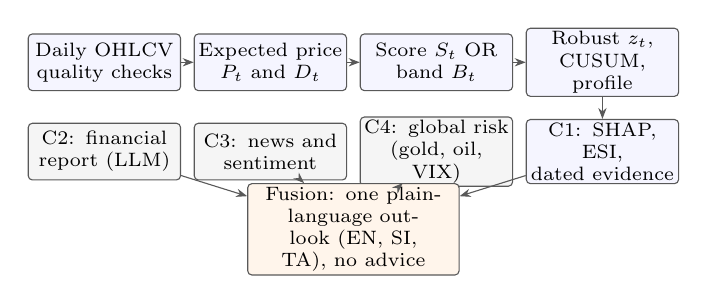
\begin{tikzpicture}[font=\scriptsize, node distance=2.2mm and 1.6mm,
  box/.style={draw=black!65, fill=blue!4, rounded corners=1.5pt, align=center, minimum height=7.2mm, text width=18.5mm, inner sep=1.2pt, font=\scriptsize},
  other/.style={box, fill=black!4},
  outb/.style={box, fill=orange!8, text width=26mm},
  arr/.style={-{Stealth[length=1.4mm]}, black!65}]
\node[box] (a) {Daily OHLCV\\quality checks};
\node[box, right=of a] (b) {Expected price\\$P_t$ and $D_t$};
\node[box, right=of b] (c) {Score $S_t$ OR\\band $B_t$};
\node[box, right=of c] (d) {Robust $z_t$,\\CUSUM, profile};
\node[other, below=4mm of a] (r) {C2: financial\\report (LLM)};
\node[other, right=of r] (n) {C3: news and\\sentiment};
\node[other, right=of n] (g) {C4: global risk\\(gold, oil, VIX)};
\node[box, right=of g] (s) {C1: SHAP, ESI,\\dated evidence};
\node[outb, below=4mm of $(n)!0.5!(g)$] (f) {Fusion: one plain-language outlook (EN, SI, TA), no advice};
\draw[arr] (a)--(b); \draw[arr] (b)--(c); \draw[arr] (c)--(d); \draw[arr] (d)--(s);
\draw[arr] (r)--(f); \draw[arr] (n)--(f); \draw[arr] (g)--(f); \draw[arr] (s)--(f);
\end{tikzpicture}
\caption{Component~1 workflow (top) and its place in the four-component system. Synthesis does not alter market calculations.}
\label{fig:workflow}
\end{figure}

\section{Experimental Design}
\emph{Stocks and provenance.} Development histories contain 3,384 JKH.N0000 and 3,314 BIL.N0000 observations, February 2012--28 August 2026. A read-only exporter attempts the current directory's listings, using split-adjusted TradingView CSELK history and CSE high/low reconciliation without modifying MongoDB. Eligibility requires 1,000 observations, a start no later than 1 January 2014, an end no earlier than 30 June 2026, and positive volume on at least 80\% of recorded final-year observations. The latter is not 80\% of all official exchange sessions. Source, exclusion and execution counts are reported separately. Seed 42 is used throughout.

\emph{A. Daily proxies.} Labels combine past-only return (97.5th percentile), volatility/volume (90th percentile) tails over 252 earlier observations with predefined stress windows. Approximately 70/10/20 chronological splits give 663 JKH and 649 BIL test observations, each with 12 positives. Ablations use validation $F_{0.5}$; the return-Z and Isolation-Forest baselines retain training-based thresholds, so tuning budgets differ. The combined alert adapts past-only thresholds during testing. F1 intervals use 2,000 moving-block replicates, block length 20~\cite{kunsch1989}; interval overlap is not a paired significance test.

\emph{B. Documented periods.} Annual refits use only preceding data, with the final 12.5\% of that history for validation. E1 covers 22 April--10 May 2019~\cite{ft_easter2019}; E2 covers 9 March--15 May 2020, including the closure~\cite{morning_covid2020}; E3 covers March--July 2022~\cite{bs_halt2022}. A nominal 2\% calibration alert budget uses 2016--2018 only; ties can make realised rates slightly exceed it. Crucially, this experiment's combined rule is standardised log-volume-score OR robust residual, allocating half the budget to each. It is not the same score-OR-band rule as Experiment A. Out-of-episode alerts are not independently verified false positives.

\emph{C. Forecasts.} Preserved three-month paths match 57 dates against persistence. Their recorded preservation date, 10 May 2026, follows the first target; preregistration is unverified. Loss-difference calculations inspired by Diebold--Mariano~\cite{diebold1995} are exploratory: these are one-origin multi-step paths, not repeated independent one-day forecasts. The application's newer 4/21/60/120-session models are separate and are not validated by this preserved-path comparison.

\emph{D. Patterns.} The three periods and an unlabelled 8 May--28 August 2026 window receive profiles. Background frequencies use non-overlapping 20/60-observation windows outside those periods. Different lengths and shared market events invalidate a simple independent-binomial enrichment claim; we report descriptive frequencies instead.

\emph{E. Across securities.} Completed-cohort aggregation compares daily F1, episode flags and outside-alert rates. Predeclared paired signed-rank comparisons with Holm correction remain exploratory because securities and share classes share companies, dates and market shocks. Incomplete execution is not presented as completed replication.

\emph{F. Planned participant evaluation.} A public versioned protocol proposes comparing chart-only and chart-plus-explanation conditions using two anonymised stocks and four counterbalanced groups. Its primary outcome is five-item comprehension; interpretation, confidence and ratings are secondary. It targets 20 adults as a pilot, not a verified power guarantee. Ethics approval and native-speaker review must precede recruitment. An approved participant dataset is not available for this manuscript; no human outcomes are reported.

\begin{figure*}[!t]
\centering
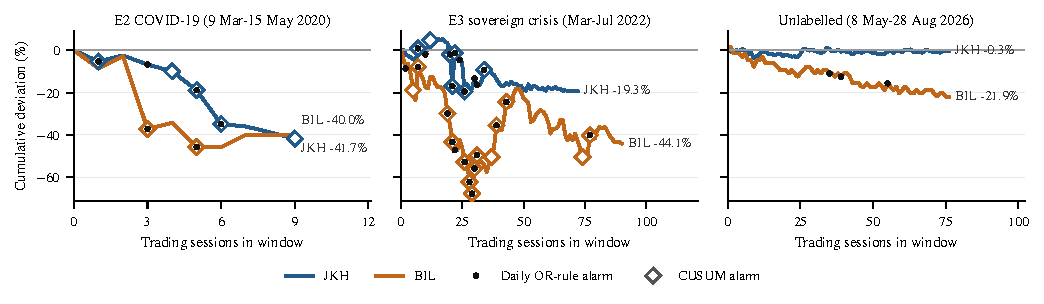
\includegraphics[width=\textwidth]{fig_pattern_monitor.pdf}
\caption{Cumulative deviation from the walk-forward expected price during two documented episodes and the unlabelled 2026 window. Dots: daily OR-rule alarms; diamonds: CUSUM alarms. BIL's slow 2026 drift raised only scattered daily alarms and no CUSUM alarm.}
\label{fig:patterns}
\end{figure*}

\section{Results}
\subsection{Daily Detection and Ablation}
Table~\ref{tab:ablation} is regenerated from the corrected rerun. Robust residuals give the largest observed F1: JKH 0.786 (95\% block-bootstrap interval 0.59--0.91), BIL 0.400 (0.00--0.67). JKH has 11 true and five false proxy alerts. Exact window centring adds one false alert relative to the earlier implementation's F1 of 0.815.

The adaptive score-OR-band rule recovers nine of 12 positives for each stock, but raises 30/163 false proxy alerts. Score-only detects zero JKH positives with 23 false alerts and three BIL positives with 166 false alerts. Its participation adjustment can amplify thin-trading observations rather than identify events.

One-step MAE does not improve on persistence: 0.1918 versus 0.1914 LKR for JKH and 0.1031 for both BIL estimates. BIL's selected blend is zero. Return-based labels consequently favour residuals that approach returns. Twelve positives, unequal baseline tuning and overlapping bootstrap intervals limit comparative claims.

\begin{table}[!t]
\caption{Reproduced Development-Stock Daily Detection (12 Proxy Positives Each)}
\label{tab:ablation}
\centering\footnotesize
\setlength{\tabcolsep}{2.7pt}
\begin{tabular}{@{}lrrrrr@{}}
\toprule
Detector & TP/FP & Pr. & Re. & F1 & 95\% CI \\
\midrule
\multicolumn{6}{l}{\textit{JKH (663 test sessions)}}\\
Adaptive score OR band & 9/30 & 0.231 & 0.750 & 0.353 & 0.15--0.54 \\
Volume score only & 0/23 & 0.000 & 0.000 & 0.000 & 0.00--0.00 \\
Band only & 5/2 & 0.714 & 0.417 & 0.526 & 0.00--0.86 \\
Unscaled $|D_t|$ & 5/2 & 0.714 & 0.417 & 0.526 & 0.00--0.86 \\
Robust $|z_t|$ & 11/5 & 0.688 & 0.917 & 0.786 & 0.59--0.91 \\
Return Z-score & 4/1 & 0.800 & 0.333 & 0.471 & 0.00--0.79 \\
Isolation Forest & 8/14 & 0.364 & 0.667 & 0.471 & 0.21--0.72 \\
\multicolumn{6}{l}{\textit{BIL (649 test sessions)}}\\
Adaptive score OR band & 9/163 & 0.052 & 0.750 & 0.098 & 0.04--0.18 \\
Volume score only & 3/166 & 0.018 & 0.250 & 0.033 & 0.00--0.08 \\
Band only & 1/0 & 1.000 & 0.083 & 0.154 & 0.00--0.44 \\
Unscaled $|D_t|$ & 1/0 & 1.000 & 0.083 & 0.154 & 0.00--0.44 \\
Robust $|z_t|$ & 3/0 & 1.000 & 0.250 & 0.400 & 0.00--0.67 \\
Return Z-score & 1/0 & 1.000 & 0.083 & 0.154 & 0.00--0.44 \\
Isolation Forest & 0/0 & 0.000 & 0.000 & 0.000 & 0.00--0.00 \\
\bottomrule
\end{tabular}

\end{table}

\subsection{Documented Stress Episodes}
The fixed-budget combined rule flags all six stock--period cases with outside-alert rates 1.93 (JKH) and 1.98 (BIL) per 100 sessions, compared with 2.05/3.72 for return Z-scores and 1.87/3.12 for robust residuals. Thus it does not minimise outside alerts for both stocks. The volume score misses one JKH and two BIL cases; EWMA misses one BIL case. CUSUM flags all six but does not consistently provide earlier warning. Three shared periods per stock support case descriptions, not independent evidence of crisis-prediction ability.



\subsection{Deviation Patterns}
Fig.~\ref{fig:patterns} uses corrected CUSUM markers rather than the mistakenly exported EWMA flags. Five of six crisis profiles receive labels: JKH volatility bursts in 2019/2022 and negative drift in 2020; BIL volatility bursts in 2019/2020. JKH's 2020 $Z_W=-13.94$ is below its reference cutoff $-1.99$.

BIL's 2022 fall of 44.1\% receives no label: $Z_W=-1.11$ does not cross $-1.31$, and scale 1.897 does not cross 1.917. Its 2026 fall of 21.9\% also remains unlabelled: $Z_W=-1.341$ is just above $-1.343$, while open share 0.842 is below 0.855. Continuous statistics therefore reveal changes that hard labels miss. JKH falls 3.9\% in 2026 but stays close to its expected path (compounded deviation $-0.3\%$). None of these profiles identifies a causal event or a recovery price.





\subsection{Held-Out CSE Listings}
\ReplicationResults
\begin{table}[!t]
\caption{Source Audit and Execution Status at Manuscript Generation}
\label{tab:inclusion}
\centering\footnotesize
\setlength{\tabcolsep}{2.7pt}
\begin{tabular}{@{}lr@{}}
\toprule
Stage & Securities \\
\midrule
Current directory listings & 302 \\
Histories exported / source exclusions & 253 / 49 \\
Eligible / data-eligibility exclusions & 202 / 51 \\
Development securities & 2 \\
Eligible held-out securities & 200 \\
Held-out runs completed / failed & 74 / 6 \\
Eligible held-out runs pending & 120 \\
\bottomrule
\end{tabular}
\parbox{\columnwidth}{\scriptsize Snapshot: 2026-10-24 14:56 UTC. The inventory is current at acquisition, not a historical point-in-time listing universe.}
\end{table}
\input{heldout_table.tex}

\subsection{User Study}
No human observations are reported. The offline kit contains consent materials, English/Sinhala/Tamil task text, a counterbalanced design and an analysis script. A browser test is software verification, not a participant trial. Its manually authored explanation paragraphs are not automatically the deployed application's output. Future recruitment requires ethics clearance and reviewed translations; any comprehension finding would apply first to these stimuli, not to the complete financial decision-support system.

\subsection{Forecasts and Explanations}
The preserved ensemble's MAE is 1.416 LKR for JKH and 0.882 for BIL, against 0.547/0.656 for persistence on the same 57 dates. This is an observed baseline win, not proof of general forecast superiority from one origin. Exploratory HAC loss-difference statistics do not remove the dependence or establish preregistration. JKH's nominal 80\% interval covers 38.6\% of outcomes; its 95\% interval covers all at mean width 8.91 LKR. High coverage alone can conceal an uninformatively wide range.

\begin{table}[!t]
\caption{Development-Stock Test-Set Surrogate Fidelity and Attribution Shares}
\label{tab:explain}
\centering\footnotesize
\setlength{\tabcolsep}{2.7pt}
\begin{tabular}{@{}llrrlr@{}}
\toprule
Stock & Target & $R^2$ & $\rho$ & Factors (\%) & ESI \\
\midrule
JKH & log(1+score) & 0.83 & 0.90 & Volume ratio 59.6; Return 31.2 & 1.00 \\
JKH & Band severity & 0.89 & 0.98 & Return 72.8; Range 13.7 & 0.98 \\
BIL & log(1+score) & -3.08 & 0.87 & Return 42.2; Volume ratio 35.7 & 1.00 \\
BIL & Band severity & 0.90 & 0.89 & Return 67.3; ATR(14) 18.4 & 1.00 \\
\bottomrule
\end{tabular}
\parbox{\columnwidth}{\scriptsize Volume score target is log(1+min(score, $10^6$)). Shares average absolute Tree-SHAP magnitudes over test rows; they are not causal effects.}
\end{table}

Table~\ref{tab:explain} is reproduced by fitting the surrogate on training/validation rows and assessing later test rows. Its target is $\log(1+\min(S_t,10^6))$, not the untransformed score. JKH fidelity is $R^2=0.827$; BIL's $R^2=-3.080$ is worse than predicting the test mean despite rank correlation 0.871. Extreme scores and distribution shift require caution rather than confident explanations.

Changing the target to volume-free band severity gives $R^2=0.895/0.902$ and shifts leading shares to daily return (72.8\%/67.3\%). Factor overlap remains high (ESI 0.978--1.000). This target-sensitivity experiment supports an algorithmic explanation for volume dominance; it does not establish market causality, explanation correctness for users, or validated interactions.

\section{Discussion and Limitations}
Three findings guide further work. Participation can qualify the reliability of an observed gap, but this study does not show that dividing by volume improves event discrimination. Robust residuals are the strongest daily signal observed on the development proxies, while continuous profiles reveal substantial declines missed by hard pattern labels. Finally, explaining a detector requires validating the surrogate against its actual target, not merely displaying stable factor names. The evidence does not yet establish improved investor understanding.

Limitations include return-defined proxies, only three shared stress periods, unequal baseline tuning and one forecast origin. Current-directory sampling can exclude delisted firms; voting/non-voting securities are not independent companies. Secondary split-adjusted histories do not establish complete corporate-action or exchange-calendar reconciliation. Source exclusions may select more available/liquid securities. Development-driven rule changes and the additional scale correction remain disclosed; their code freeze is not prospective market validation. No participant, comprehension, causal or profitability study is completed.

For reproducibility, \url{https://github.com/it21296482/R26-IT-076} preserves the earlier and corrected methods, source/exclusion receipts and pre-extension code snapshot. S.~A.~H.~Samarathunga contributes market modelling and validation; K.~C.~S.~Fernando report interpretation; Harithra~K news/sentiment; and T.~G.~R.~N.~S.~Wijesooriya explained global risk. Kapila Dissanayaka and Mahima Weerasinghe supervise the project. The other integrated contributions are not independently evaluated here. Outputs support investigation, not trading advice.

\section{Conclusion}
The evaluated workflow makes deviations, participation, alerts and explanation limitations inspectable. Its daily volume adjustment is not superior to robust residuals on the development proxies, and persistence beats the preserved forecast paths. Pattern profiles add context but their labels miss substantial declines; continuous statistics must remain visible. \ReplicationConclusion\ Participant evaluation remains planned, so no comprehension gain is claimed. Independent event adjudication, matched tuning, repeated prospective forecast origins and approved comprehension studies are needed before broader claims.

\bibliographystyle{IEEEtran}
\bibliography{refs}

\end{document}
